\chapter{Introduction and Overview}
\paragraph*{}
The project, “Collective Transport using Decentralised Swarm Robotics,” aims to pioneer a new approach to robotic collaboration by enabling decentralised control for tasks such as object transportation in unstructured environments. Traditional centralised systems, like those in RoboCup Soccer, have dominated the field for decades but face limitations such as single points of failure and reliance on powerful centralised servers. This project seeks to address these challenges by leveraging decentralised swarm robotics, which ensures robust, scalable, and efficient operations without dependency on a single control unit.
 
A core objective of the project is to develop a system where three robots can simultaneously map their environment, communicate with one another, and collaborate to transport an object from point A to point B in a synchronised manner. This involves the robots autonomously detecting an object, localising themselves in the environment, and coordinating their movements to ensure seamless and efficient transport. This goal demonstrates the potential of decentralised swarm robotics for highly coordinated tasks that require precise communication and execution. See figure \ref{fig:robot-transport-sim} for an simulation of the project's goal using the simulation.
See figure \ref{fig:robot-transport-draw} for an illustration of the project's goal using a drawing 

\begin{figure} [H]
    \centering
    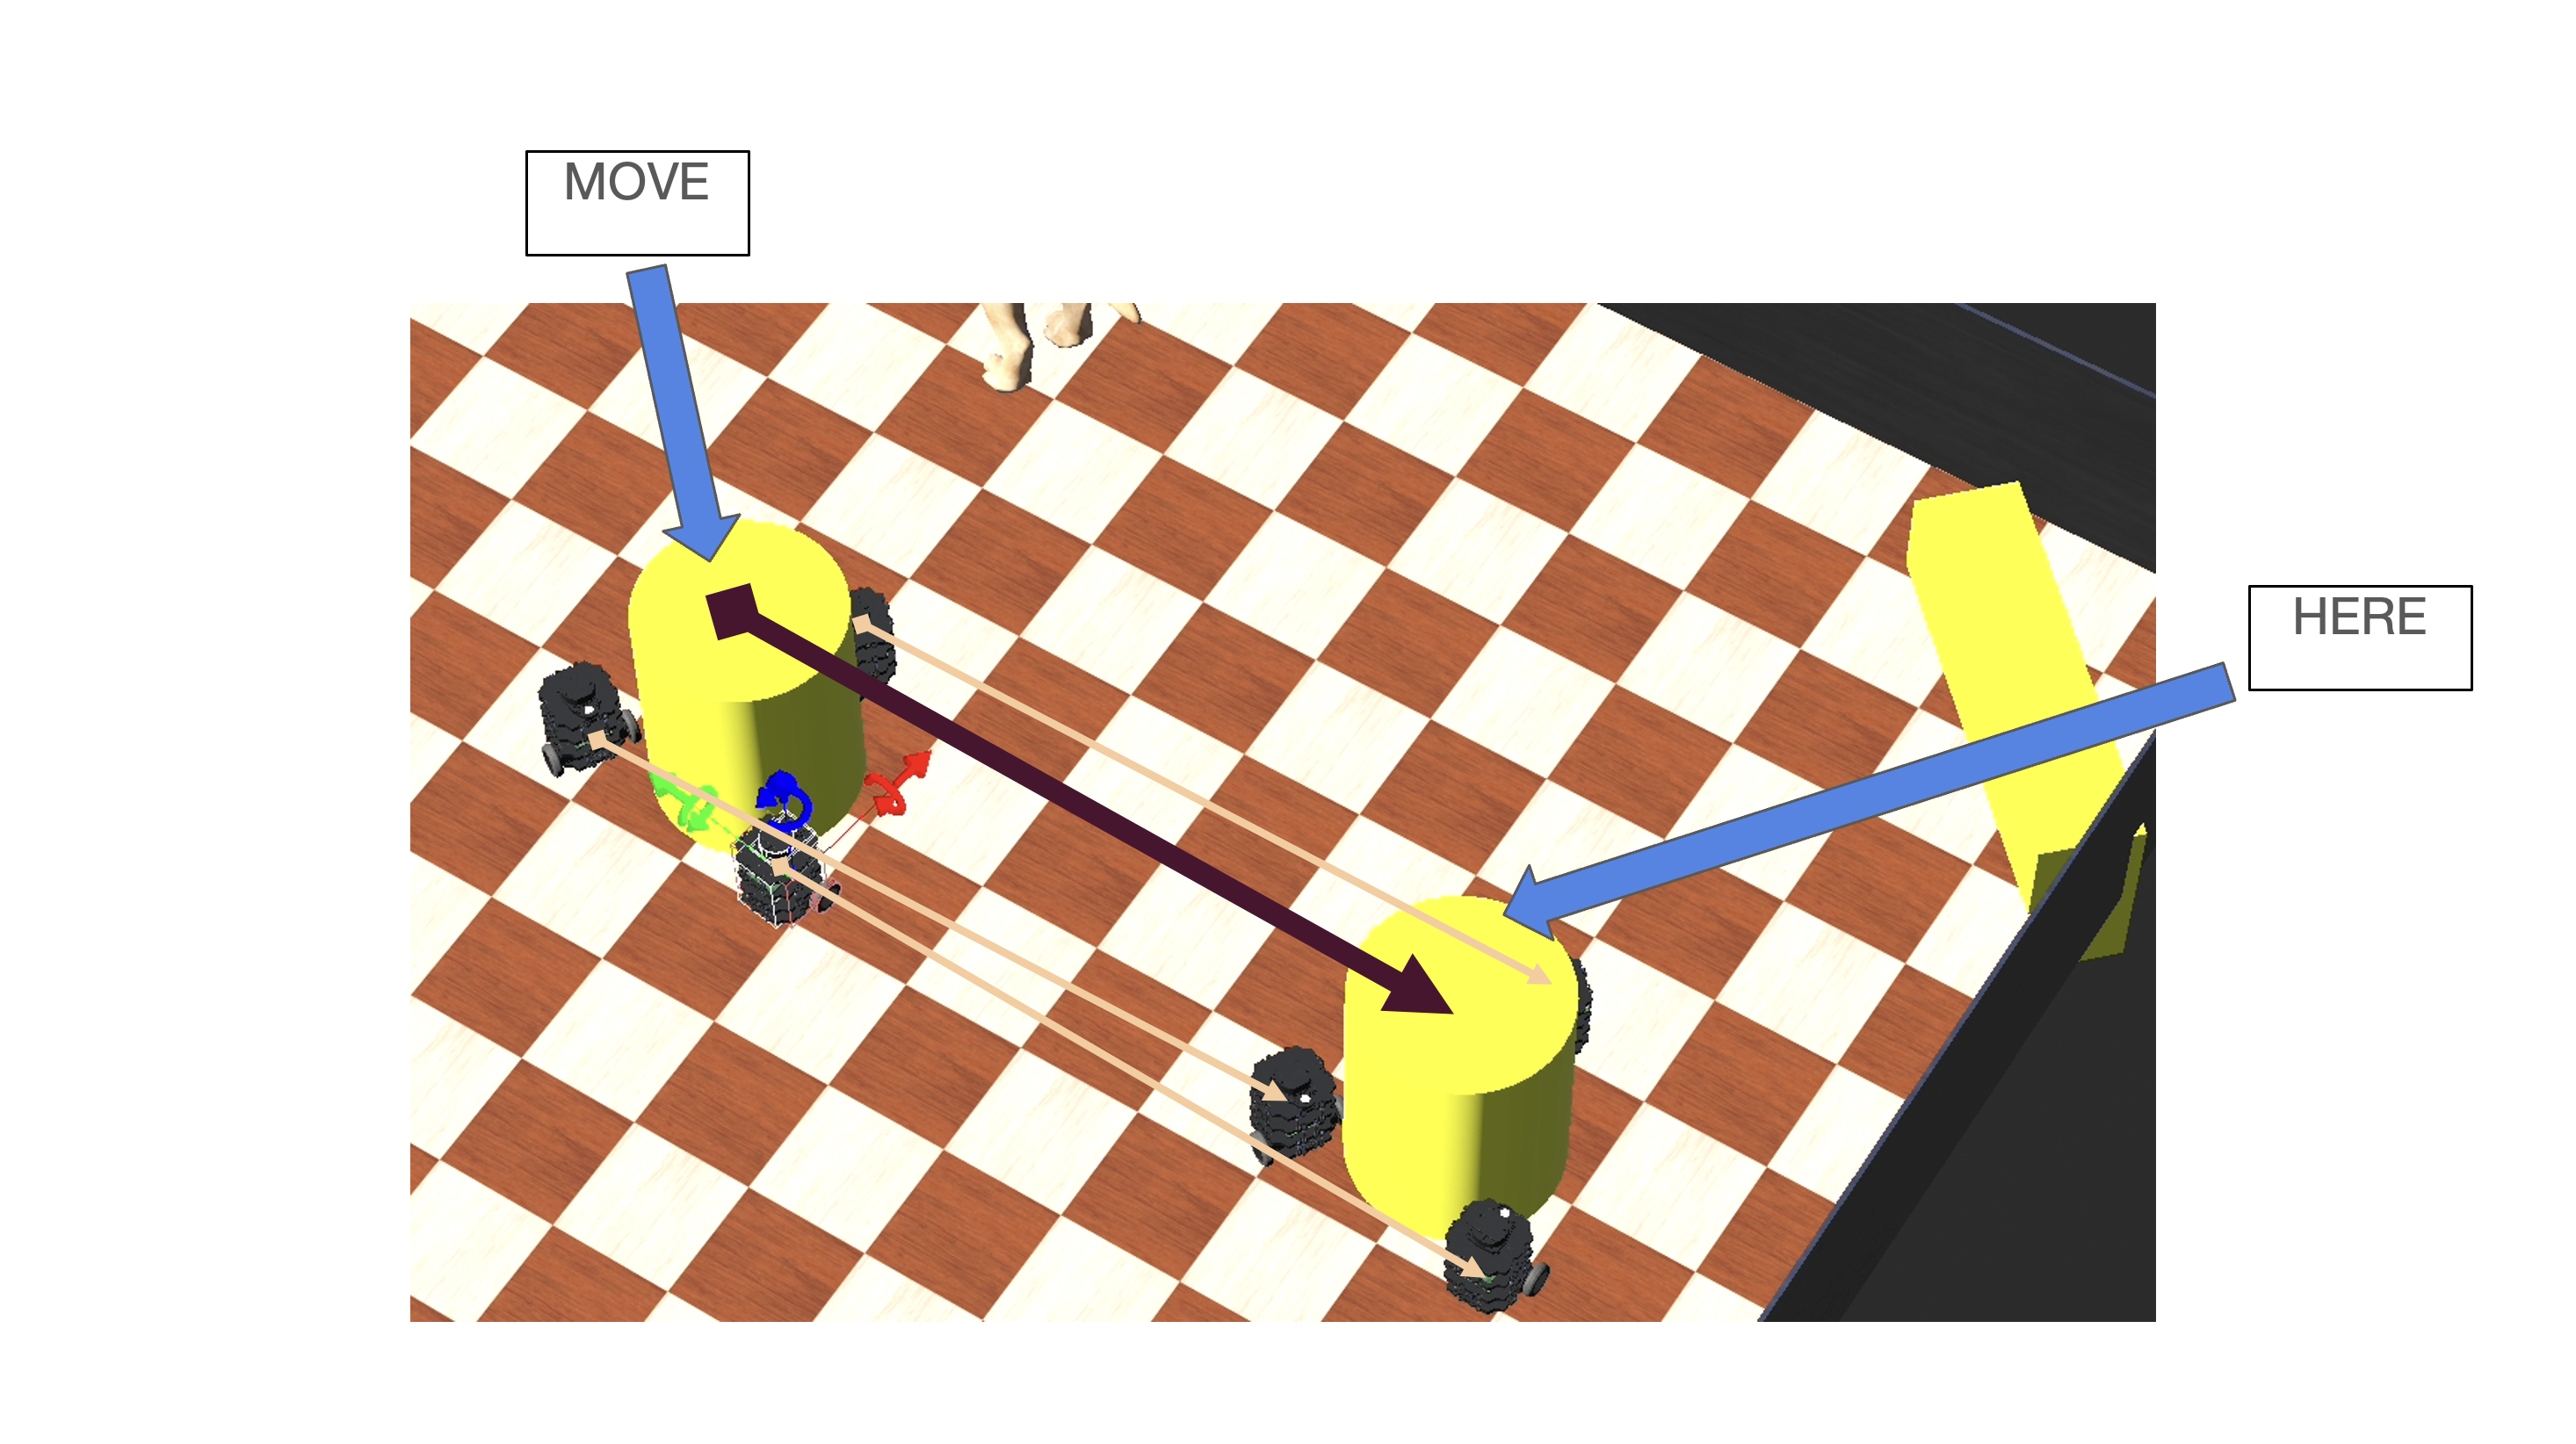
\includegraphics[width=1.0\linewidth]{assets/images/introduction/robot-transport-sim.png}
    \caption{Illustration of the project's goal: three robots transporting an object using simulation}
    \label{fig:robot-transport-sim}
\end{figure}
\begin{figure} [H]
    \centering
    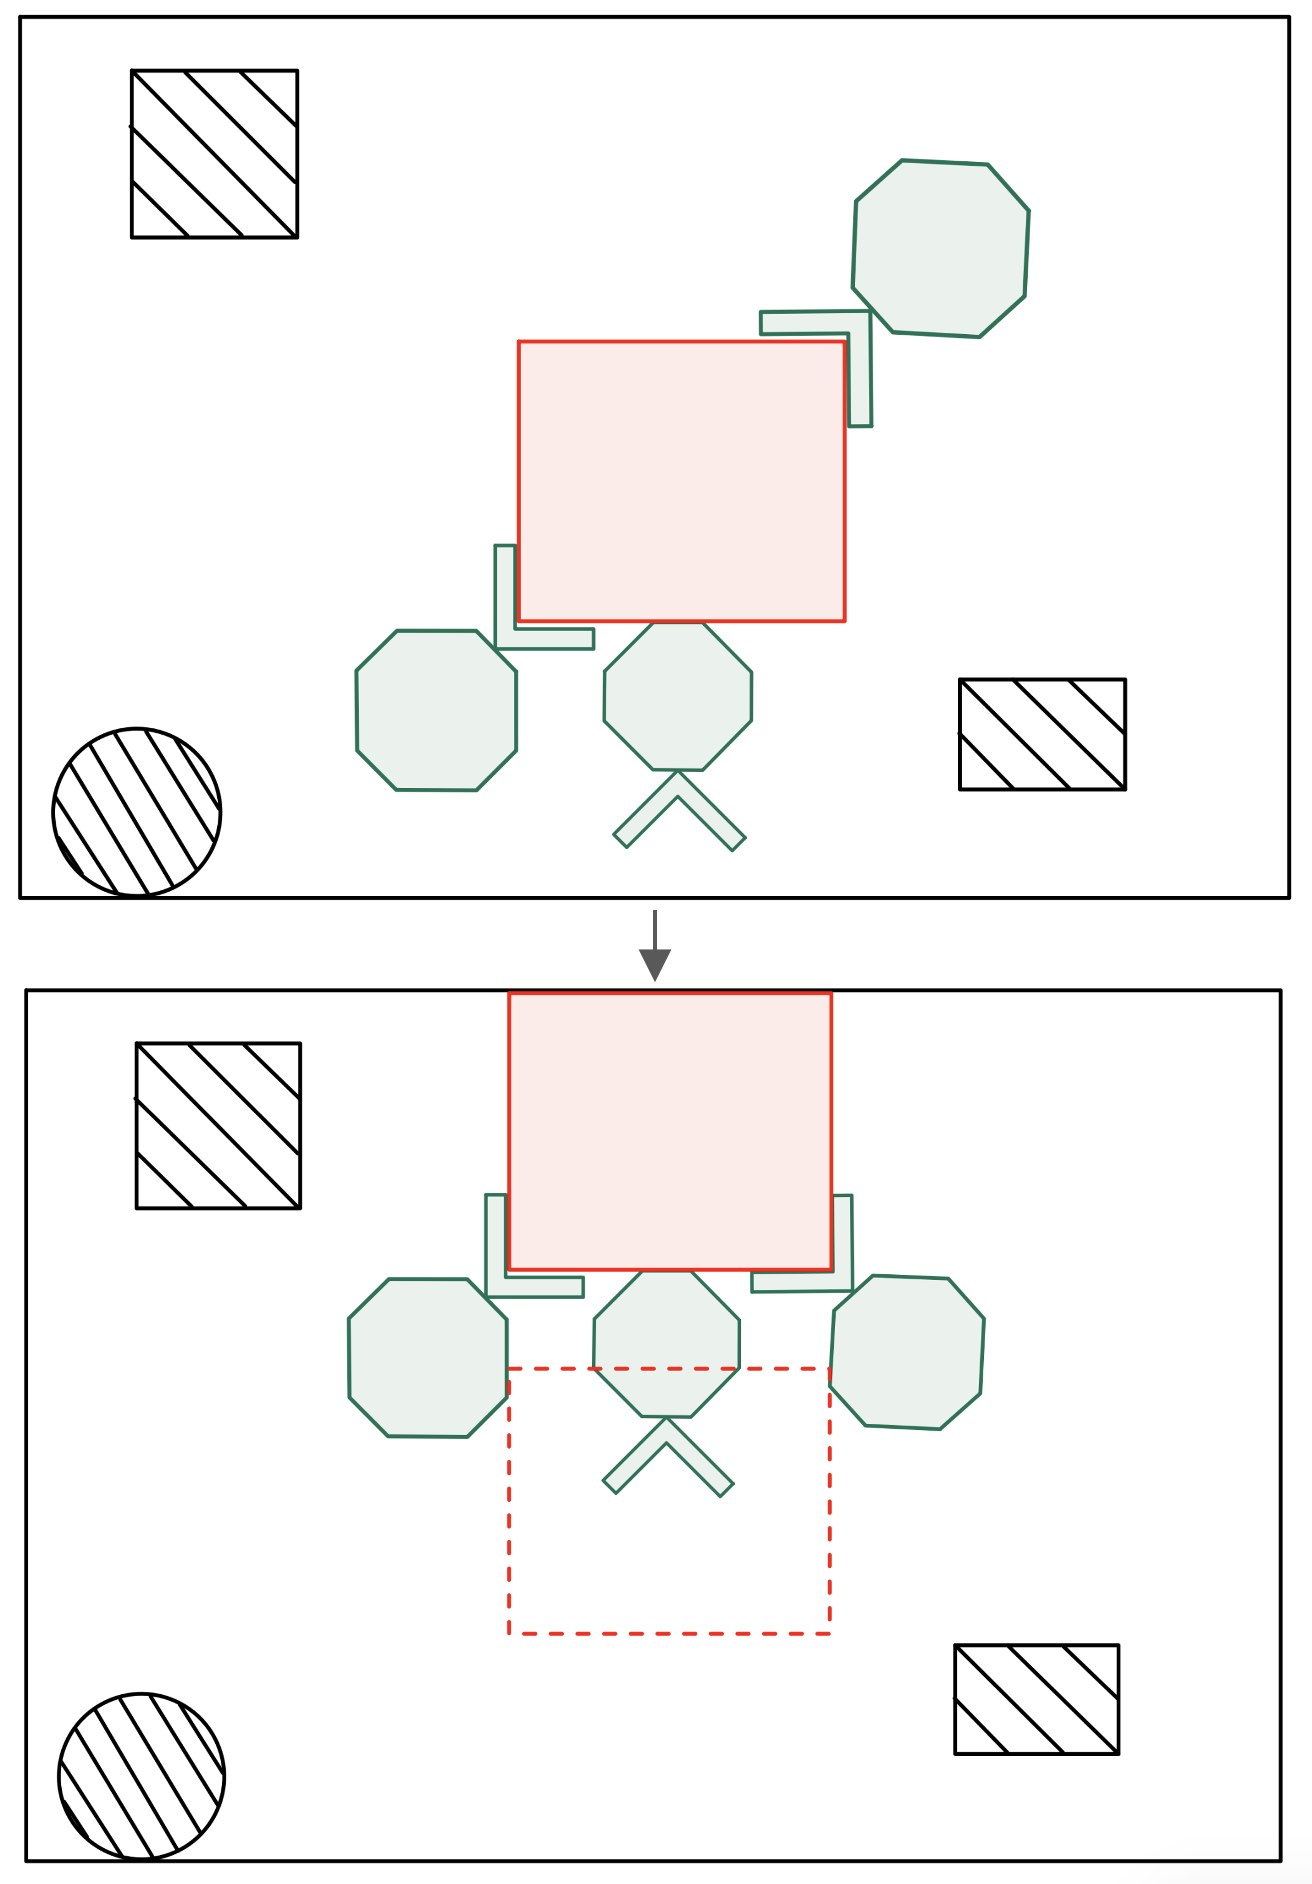
\includegraphics[width=0.75\linewidth]{assets/images/introduction/robot-transport-draw.png}
    \caption{Illustration of the project's goal: three robots transporting an object using a drawing}
    \label{fig:robot-transport-draw}
\end{figure}

In real-world applications, this approach holds transformative potential, particularly in warehouse logistics and search-and-rescue operations. The decentralised model offers resilience and adaptability, making it suitable for scenarios where centralised systems may falter. Moreover, this technology aligns with Thailand’s growing need for innovative solutions in robotics, showcasing a shift towards decentralised systems that can operate independently without a centralised power hub. This represents a vision for the future of robotics, where hardware and computation costs decrease, enabling accessible and scalable robotic systems.

The project development is divided into two phases:
	1.	Phase 1: Exploration of foundational modules, including communication protocols, object detection via computer vision, and localisation. While the original plan included SLAM, it was deprioritised due to its limited necessity in the simulation phase. However, the team actively studied SLAM in preparation for its integration in Phase 2. A significant focus was placed on ensuring the robustness of these individual modules, validated through simulations in Webots, which provided a cost-efficient, risk-free environment.
	2.	Phase 2: Integration of these foundational modules into a working prototype of robots navigating their environment. This phase also incorporates SLAM, advanced robot formations, and initial hardware configurations. The ultimate goal is to transition from simulation to real-world applications, with the simulation results guiding the hardware design.

The success of the project is measured not only by the accuracy and control of individual robots but also by the robustness of their communication and coordination. Metrics include the ability to resolve edge conditions, such as simultaneous object detection or potential collision paths, and the effectiveness of decentralised decision-making. Overhead cameras verify the robots’ positional accuracy, ensuring that simulated and real-world performance align

This report highlights the project’s accomplishments, including completed tasks like communication, object detection, and localisation, alongside the progress of module integration. It also underscores the importance of simulation as a foundation for hardware development and presents a roadmap for achieving decentralised, collaborative transport systems. Through this effort, the project aims to establish a framework that not only advances robotics technology but also addresses challenges specific to Thailand, paving the way for future innovations in swarm robotics.

\paragraph*{}
This midpoint report aims to highlight the progress of our project throughout the whole semester, with the evaluating criteria being the team's contributions alongside the pace in comparison to the ideal schedule. The ideal project timeline is presented with the Gantt Chart below. (Figure \ref{fig:gantt-chart})

\begin{figure} [H]
    \centering
    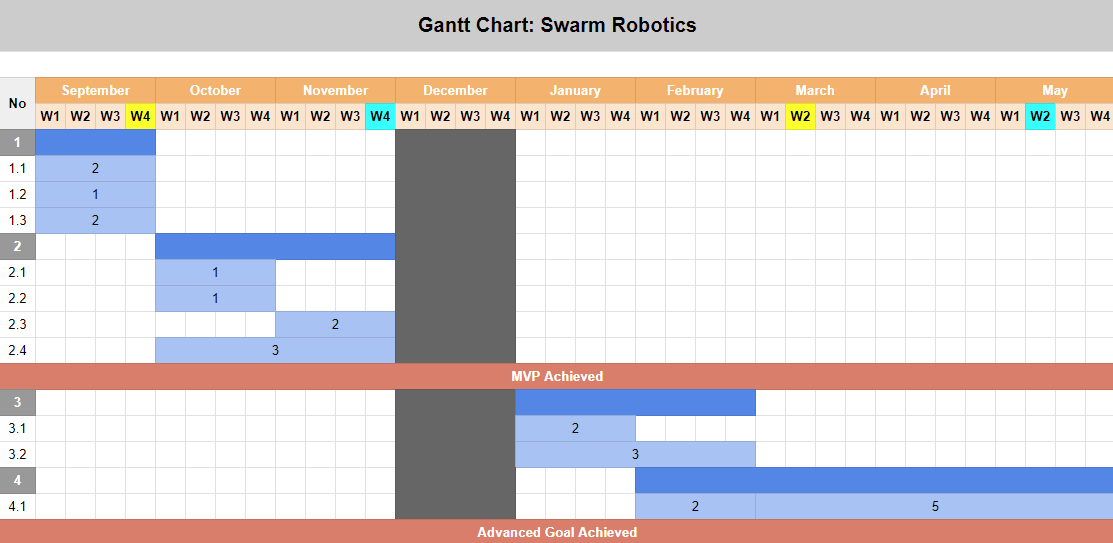
\includegraphics[width=1\linewidth]{assets/images/introduction/gantt_chart.png}
    \caption{Project Gantt Chart}
    \label{fig:gantt-chart}
\end{figure}

\paragraph*{Current Gantt Chart and Progress:}
\begin{description}
    \item[Phase 1: Simulation and Fundamental Modules]
    
    \item 1.1. Communication -- \textit{Completed}  
    Achieved seamless coordination between robots using an infrared-based communication system, with a consensus algorithm to resolve conflicts during simultaneous detections or task assignments.

    \item 1.2. Object Detection using Computer Vision -- \textit{Completed}  
    Developed a 2D object detection system with OpenCV for identifying the target (a yellow cylinder), aligning bounding boxes, and calculating distances accurately.

    \item 1.3. Localisation -- \textit{Completed}  
    Implemented wheel odometry with encoders and differential drive kinematics to update robot positions reliably.

    \item 2.1. Simple Robot Formation -- \textit{Completed}  
    Enabled basic formation control, allowing robots to form equilateral shapes and navigate in coordination.

    \item 2.4. Combination of Individual Modules in Simulation -- \textit{Completed}  
    Integrated communication, object detection, and localisation modules into a working prototype in the simulation.

    \item 2.2. Simultaneous Localisation and Mapping (SLAM) -- \textit{In progress}  
    Actively working on GraphSLAM, focusing on creating initial graphs, loop closure, and error function refinement to improve mapping accuracy.

    \item[Phase 2: Transition to Hardware and Advanced Features]

    \item 2.3. Hardware -- \textit{In progress}  
    Transitioning simulation modules to hardware, including:
    - Jetson installation with optimised configurations.
    - Testing closed-loop control for BLDC motors.
    - Preparing hardware communication systems for decentralised operations.

    \item 3.1. Coordinated Gripping -- \textit{To do}  
    Develop an end-effector for gripping and securing objects during collaborative transport.

    \item 3.2. Advanced Robot Formation -- \textit{To do}  
    Implement dynamic formation control to adapt to environmental changes and enhance navigation.

    \item 4.1. Hardware -- \textit{To do}  
    Transition the full system to physical robots, focusing on advanced motor control, sensor calibration, and hardware-based object detection.
\end{description}